%compiling with XeLaTeX
\documentclass[twoside,11pt,abstracton]{scrreprt}

%personel data
\title{Differentialgeometrie I}
\author{Dr. Anna Siffert}
\date{Sommersemester 2018}


%math and theorems
\usepackage{amsmath}
\usepackage{amssymb}
\usepackage[amsmath,thmmarks,hyperref]{ntheorem}
\usepackage{mathtools}
\usepackage{dsfont}
\usepackage[arrow, matrix, curve]{xy}

%language settings and microtype
\usepackage{fontspec} 
\setmainfont{Palatino}
\setsansfont{Optima}
\setmonofont[Scale=MatchLowercase]{Menlo}

\usepackage{polyglossia}
\setmainlanguage{german}
\setotherlanguages{english}
\usepackage{microtype}

%useful packages
\usepackage{geometry}
\usepackage{xcolor}
\usepackage{graphicx}
\usepackage{float}
\usepackage{fancyhdr}
\usepackage{csquotes}
\usepackage{blindtext}
\usepackage{todonotes}
\usepackage{booktabs}
\usepackage{array}
\usepackage[labelfont=bf]{caption}
\usepackage{wrapfig}
\usepackage{physics}

%geometry
\geometry{
	width=150mm,
	bindingoffset=7mm,}

%color settings
\definecolor{myred}{RGB}{196,19,47} 
\definecolor{myblue}{RGB}{0,139,139}


%for empty pages at the beginning of the document
\def\blankpage{%
	\clearpage%
	\thispagestyle{empty}
	\addtocounter{page}{-1}
	\null%
	\clearpage}

% Page layout for beginning of chapter
\fancypagestyle{plain}{%
	\fancyhf{}  % clear all header and footer fields 
	\fancyfoot[C]{- \thepage\hspace{3pt}-} 
	\renewcommand{\headrulewidth}{0pt}
	\renewcommand{\footrulewidth}{0pt}}

%page layout for the other pages
\pagestyle{fancy}
\fancyhf{}
\fancyhead[LE]{\textit{\nouppercase{\leftmark}}}
\fancyhead[RO]{\textit{\nouppercase{\rightmark}}}
\fancyfoot[C]{- \thepage\hspace{3pt}-}
\renewcommand{\headrulewidth}{0.2pt}
\renewcommand{\footrulewidth}{0pt}

% titles and stuff
\setkomafont{chapter}{\normalfont\bfseries\huge}
\setkomafont{section}{\normalfont\bfseries\LARGE}
\setkomafont{subsection}{\normalfont\bfseries\large}
\setkomafont{title}{\normalfont\bfseries\Large}
\setkomafont{author}{\normalfont\bfseries\Large}
\setkomafont{date}{\normalfont\bfseries\Large}

%nice boxes
\usepackage[many]{tcolorbox}    
\newtcolorbox{mybox}[1]{%
	tikznode boxed title,
	enhanced,
	arc=0mm,
	interior style={white},
	attach boxed title to top center= {yshift=-\tcboxedtitleheight/2},
	fonttitle=\large\bfseries,
	colbacktitle=white,coltitle=black,
	boxed title style={size=normal,colframe=white,boxrule=0pt},
	title={#1}}

%proofs,defs ...

%Theorems
\theoremstyle{marginbreak}
\theoremheaderfont{\normalfont\bfseries}
\theorembodyfont{\slshape} 
\theoremseparator{}
\newtheorem{satz}{Satz}[chapter]

%Lemma
\theoremstyle{changebreak} 
\theoremindent0.5cm 
\theoremseparator{}
\newtheorem{lem}[satz]{Lemma}

%Helping lemma, Mathieu, Q's been here
\theoremstyle{changebreak} 
\theoremindent0.5cm 
\theoremseparator{}
\newtheorem{hlem}[satz]{Hilfslemma}

%Corolarys
\theoremindent0cm 
\theoremseparator{}
\newtheorem{kor}[satz]{Korollar}

%Examples
\theoremstyle{break} 
\theorembodyfont{\upshape} 
\theoremseparator{} 
\newtheorem{bsp}[satz]{Beispiel}

%Comments
\theoremstyle{plain} 
\theorembodyfont{\upshape} 
\theoremseparator{:} 
\newtheorem*{bem}[satz]{Bemerkung}

%Definitions
\theoremstyle{break}
\theorembodyfont{\slshape} 
\theoremseparator{} 
\newtheorem{defs}[satz]{Definition}

%Proofs
%\theoremheaderfont{\normalfont} %falls es nicht dick gedruckt sein soll
\theoremstyle{nonumberbreak}
\theoremseparator{} 
\theoremsymbol{\ensuremath{\square}}
\newtheorem{bew}[satz]{Beweis:}

%bibliography
\usepackage[
style=numeric-comp,
backend=biber,
maxnames=10,
maxcitenames=2,
isbn=false,
date=year,
url=false,
doi=false
]{biblatex}
\bibliography{bibliography/diffgeo-bib}

%appendix
\usepackage[toc,page]{appendix}

%killing indent
\setlength{\parindent}{0pt}

%always use hyperref at the end of the preamble!
\usepackage[colorlinks=True]{hyperref}
\hypersetup{allcolors=myred}

%useful new defintions and stuff

\newcommand{\R}{\mathbb{R}}	%simplify R^n
\newcommand{\set}[1]{\left\{#1\right\}}	%siplify sets
\newcommand{\difM}{differenzierbare Mannigfaltigkeit}		%abbreveiate "differenzierbare Mannigfaltigkeit"
\renewcommand{\d}{{\operatorname{d}}}		%differentiial operator





% commands thomas
\newcommand{\Index}[1]{#1\index{#1}}
\newcommand*{\quelle}[1]{\par\footnotesize Quelle:~\href{#1}{#1}}
\newcommand{\im}{\mathrm{i}}
\newcommand{\e}{\mathrm{e}}
\newcommand{\mfk}{\mathcal{M}}
\newcommand{\mfka}{\mathcal{N}}
\newcommand{\atlas}{\mathcal{A}}
\newcommand{\rn}{\mathbb{R}^n}
\newcommand{\evat}{\vert\big}
\newcommand{\cinf}{C^\infty}
\newcommand{\tspace}[1]{T_{#1} \mathcal{M}}
\newcommand{\covd}{\mathrm{D}}
%\renewcommand{\pi}{\uppi}
\renewcommand{\epsilon}{\varepsilon}
\DeclareMathOperator{\id}{id}
\DeclareMathOperator{\supp}{supp}
\DeclareMathOperator{\diff}{Diff}
\DeclareMathOperator{\rang}{Rang}




\begin{document}
	
%title, abstract and toc	 
\pagenumbering{roman} %start roman numbering before main text
% !TeX root = ..//diffgeo_main.tex
\begin{titlepage}
	\begin{center}
		\makeatletter
		
		\thispagestyle{empty}
		
		\Huge\textbf{\@title} \\
		\vspace{5mm}
		\Large\textbf{ gehalten von \@author} \\
		\large{im \@date} \\
		\vspace{5mm}
		\large{an der} \\
		\Large\textbf{Ruprecht-Karls-Universität Heidelberg} \\
		\vfill
		\begin{figure}[H]
			\centering
			\includegraphics*[width=0.6\textwidth]{figures/logo-uni-hd-small}
		\end{figure}
	    \vfill
		\Large
		In \LaTeX \ gesetzt von \\ 
		\vspace{3mm}
		\bfseries{
		Mathieu Kaltschmidt
		\& 
		Quirinus Schwarzenböck}\\ 	
	   \vfill
	   \normalfont
	   aktueller Stand: \  \textit{\today}
	   \vfill
		\makeatother
	\end{center}
\blankpage
\end{titlepage}

{\renewcommand{\headrulewidth}{0pt} % kill headrule for abstract and toc
	\addcontentsline{toc}{chapter}{Vorwort}
	% !TeX root = ..//diffgeo_main.tex
\makeatletter

\begin{figure}[H]
\flushright
\includegraphics[width=0.4\textwidth]{figures/logo-uni-hd}
\end{figure}
\vspace{-30mm}
\begin{flushleft}	
\textbf{\LARGE\@title} \\
\vspace{0.5cm}
\Large\@author \\
\end{flushleft}
\vspace{5mm}
\rule{\textwidth}{0.2pt}

\makeatother

\vfill

{\let\raggedsection\centering
\section*{Vorwort}
Bei diesen Vorlesungsnotizen handelt es sich um kein offizielles Skript, sondern lediglich um die Umsetzung des Vorlesungsmitschriebs in \LaTeX. \\
Für die Vollständigkeit \& Richtigkeit des Inhalts wird deshalb \bfseries keine Gewährleistung \normalfont übernommen. \\
Bei Fragen, Korrekturen und Verbesserungsvorschlägen freuen wir uns über eine Nachricht.\footnote{Mail an \href{mailto:M.Kaltschmidt@stud.uni-heidelberg.de}{M.Kaltschmidt@stud.uni-heidelberg.de}
oder
\href{mailto:T.Ackermann@stud.uni-heidelberg.de}{T.Ackermann@stud.uni-heidelberg.de}	
} \\
Die Dozentin Frau Dr. Siffert empfiehlt die nachfolgende Literatur zur Vertiefung des in der Vorlesung behandelten Stoffs:

% books and more
\nocite{*}
\printbibliography[heading=none]

 Eine Inhaltsübersicht der in der Vorlesung behandelten Themen befindet sich auf der nächsten Seite.

\vfill

\blankpage
	\tableofcontents
	\blankpage}
}
%main content
\setcounter{tocdepth}{1}
\pagenumbering{arabic} % now set main numbering to arabic

%lectures
	% !TeX root = ..//diffgeo_main.tex
\chapter{Differenzierbare Mannigfaltigkeiten}
\section*{Worum geht es in der Differentialgeometrie?}
Die zentralen Objekte der Differentialgeometrie sind Mannigfaltigkeiten. Das Ziel ist es, Analysis und Geometrie auf solchen Mannigfaltigkeiten zu betreiben. \\
Wir beginnen zunächst einmal mit einer kurzen Gegenüberstellung der bereits bekannten Konzepte aus dem $\mathbb{R}^n$ mit den korrespondierenden Begriffen der Differentialgeometrie, welche wir in den kommenden Vorlesungen noch genauer kennenlernen werden.

%Vergleich
\begin{figure}[H]
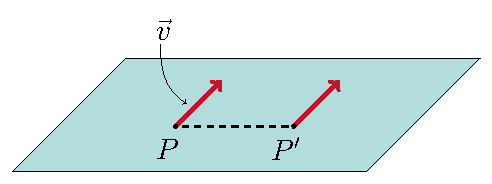
\includegraphics[scale=0.8]{figures/tikz/plane.pdf}
\hspace{2cm}
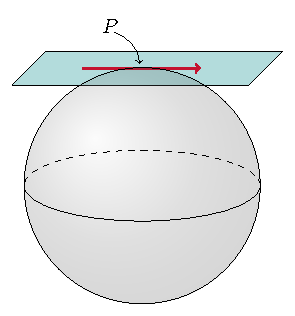
\includegraphics[scale=0.9]{figures/tikz/sphere_with_plane.pdf}
\end{figure}

\begin{figure}[H]
\centering
\begin{tabular}{>{\centering}p{.45\textwidth} | >{\centering}p{.45\textwidth}} 
$\mathbb{R}^n$ \vspace{5pt} & $\Huge\mathcal{M}$  \vspace{5pt} \tabularnewline \hline 
\vspace{5pt} Parallelverschiebung & \vspace{5pt} Begriff des Zusammenhangs\tabularnewline 
\vspace{5pt} Gerade = kürzeste Verbindung & \vspace{5pt} Konzept der Geodätischen \tabularnewline 
\vspace{5pt} flacher Raum & \vspace{5pt} gekrümmter Raum \tabularnewline 
\vspace{5pt} Skalarprodukt & \vspace{5pt} Riemannsche Metrik \tabularnewline 
\end{tabular}
\end{figure}
\section{Definitionen}
Um differenzierbare Mannigfaltigkeiten definieren zu können wiederholen wir zunächst die Definition eines topologischen Raumes. \\
\phantom{.}\\
\bfseries Erinnerung: \normalfont $M \subseteq \mathbb{R}^n$ offen, wenn $\forall p \in U \ \exists \ \varepsilon>0$, sodass $B_{\varepsilon}(p) \subset U$. Dieser Begriff von Offenheit heißt \textit{euklidische Topologie} \normalfont und erfüllt:
\begin{enumerate}
\item[i)] $\emptyset, \mathbb{R}^n$ offen
\item[ii)] $U, V \subset \mathbb{R}^n$ offen $\Rightarrow U \cap V$ offen in $\mathbb{R}^n$
\item [iii)] $U_i, i \in $ I offen in $\mathbb{R}^n \Rightarrow \bigcup\limits_{i \in \text{I}} U_i \subset \mathbb{R}^n$ offen
\end{enumerate} 


\begin{figure}[H]
\centering
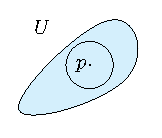
\includegraphics[scale=1.4]{figures/tikz/openset.pdf}
\caption{Offene Menge}
\label{img:offenemenge}
\end{figure} 

\begin{defs}[Topologischer Raum]
Ein topologischer Raum ist eine Menge $X$ zusammen mit einer Menge $\mathcal{O} \subset \mathcal{P}(X)$, sodass:
\begin{enumerate}
	\item[i)] $\emptyset, X \in \mathcal{O}$
	\item[ii)] $U, V \in \mathcal{O} \Rightarrow  U \cap V \in \mathcal{O}$
	\item [iii)] $U_i \in \mathcal{O} \Rightarrow\bigcup\limits_{i \in \text{I}} U_i \in \mathcal{O}$
\end{enumerate} 
\end{defs}
\begin{bsp}
\begin{enumerate}
	\item[a)] $( X, \mathcal{O} = \mathcal{P}(x) )$
	\item[b)] $N \subset X$ Teilmenge. Dann ist auch $(N,\mathcal{O}_1)$ ein topologischer Raum, wobei $\mathcal{O}_1$ wie folgt gegeben ist:\\
	\center{$V \in \mathcal{O}_1 \Leftrightarrow \ \exists \ U \in \mathcal{O}$, sodass $V= N \cap U$}
\end{enumerate}
%\begin{figure}[h]
%\centering
%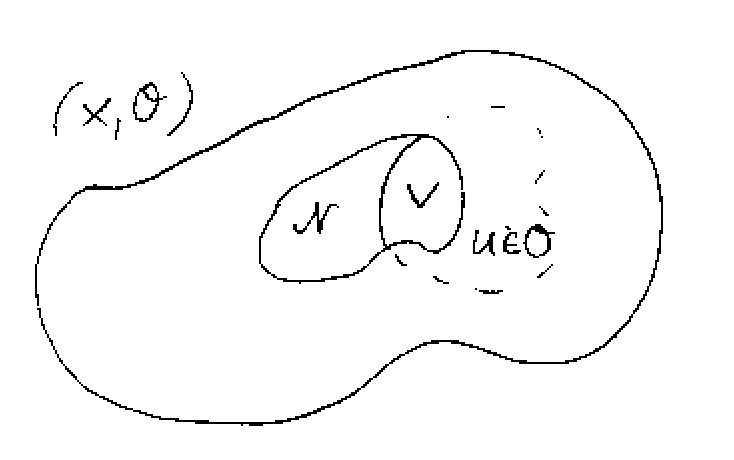
\includegraphics[width=0.35\linewidth]{figures/scan/teilmengetopologie.png}
%\label{img:teilmengetopologie}
%\end{figure}
Teilmengen topologischer Räume sind topologische Räume.
\end{bsp}

\begin{defs}[Topologische Mannigfaltigkeiten]
Eine topologische Mannigfaltigkeit ist ein topologischer Raum $\mathcal{M}$ der Dimension $n$ mit folgenden Eigenschaften:
\begin{enumerate}
	\item[i)] $\mathcal{M}$ ist hausdorffsch. Das heißt $\forall \ p, q \in \mathcal{M}$ mit $p \neq q \  \exists$ \ zwei disjunkte, offene Umgebungen $U \in p$ und $V \in q$ wobei $U, V \in \mathcal{O}$
\begin{figure}[H]
\centering
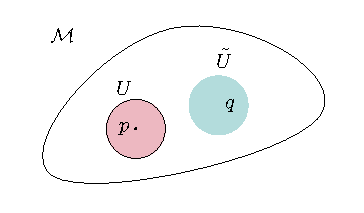
\includegraphics[width=0.4\linewidth]{figures/tikz/hausdorff.pdf}
\caption{Hausdorff'sche Eigenschaft}
\label{img:hausdorff}
\end{figure} 	
	\item[ii)] \textbf{2. Abzählbarkeitsaxiom}  \\
	$\mathcal{M}$ hat eine abzählbare Basis der Topologie, das heißt es existieren abzählbar viele Mengen $\{U_1, \dots, U_k, \dots\}$ offener Teilmengen mit $U_i \in \mathcal{O}$, sodass $\forall p \in \mathcal{M}$ und alle Umgebungen $U$ von $p$ gibt es ein $K$ sodass $p \in U_k \subseteq U$.
	\item [iii)] $\mathcal{M}$ ist homöomorph zu $\mathbb{R}^n$, das heißt $\forall p \in \mathcal{M}$ existiert eine Umgebung $U$ von $p$ und ein \bfseries Homöomorphismus \normalfont $X: U \rightarrow V \subseteq \mathbb{R}^n$ (offen).
\end{enumerate} 
\end{defs}
\begin{minipage}[H]{.8\textwidth}
\begin{defs}[Karte, Atlas]
	Das Paar $(X, U)$ heißt \textbf{Karte} von $\mathcal{M}$ um $p$. \\
	Eine Menge $\mathcal{A} = \{(x_{\alpha},U_{\alpha})_{\alpha \in \mathcal{A}}\}$ von Karten heißt \textbf{Atlas} von $\mathcal{M}$, falls \\
	\begin{align}
	\bigcup\limits_{\alpha \in \mathcal{A}} = \mathcal{M}
	\end{align}
\end{defs}
\end{minipage}
\hspace{1cm}
\begin{minipage}[H]{.2\textwidth}
\vspace{-0.5cm}
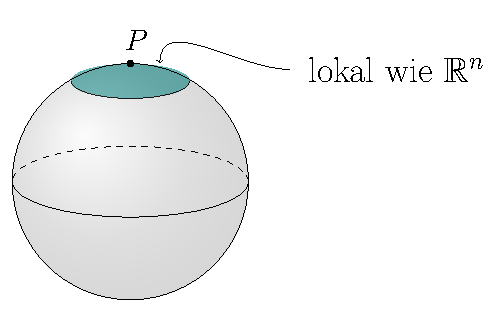
\includegraphics[scale=0.5]{figures/tikz/sphere_local_rn}
\end{minipage}


Topologische Mannigfaltigkeiten sind die Grundbausteine. Nun wollen wir auf diesen Mannigfaltigkeiten Geometrie betreiben. Dafür benötigen wir mehr Struktur. Wir wollen die differenzierbare Struktur des $\mathbb{R}^n$ auf unseren Mannigfaltigkeiten "holen".

\begin{defs}[Kartenwechsel]
Seien $x_{\alpha}$ und $x_{\beta}$ zwei Karten, dann ist der Kartenwechsel wie folgt definiert: \\
\begin{align}
x_{\alpha}\circ x_{\beta}^{-1}: x_{\beta}(U_{\alpha}\cap U_{\beta}) \rightarrow x_{\alpha}(U_{\alpha}\cap U_{\beta}) \subseteq \mathbb{R}^n
\end{align}
Dies ist ein Homöomorphismus.

\begin{figure}[H]
\centering
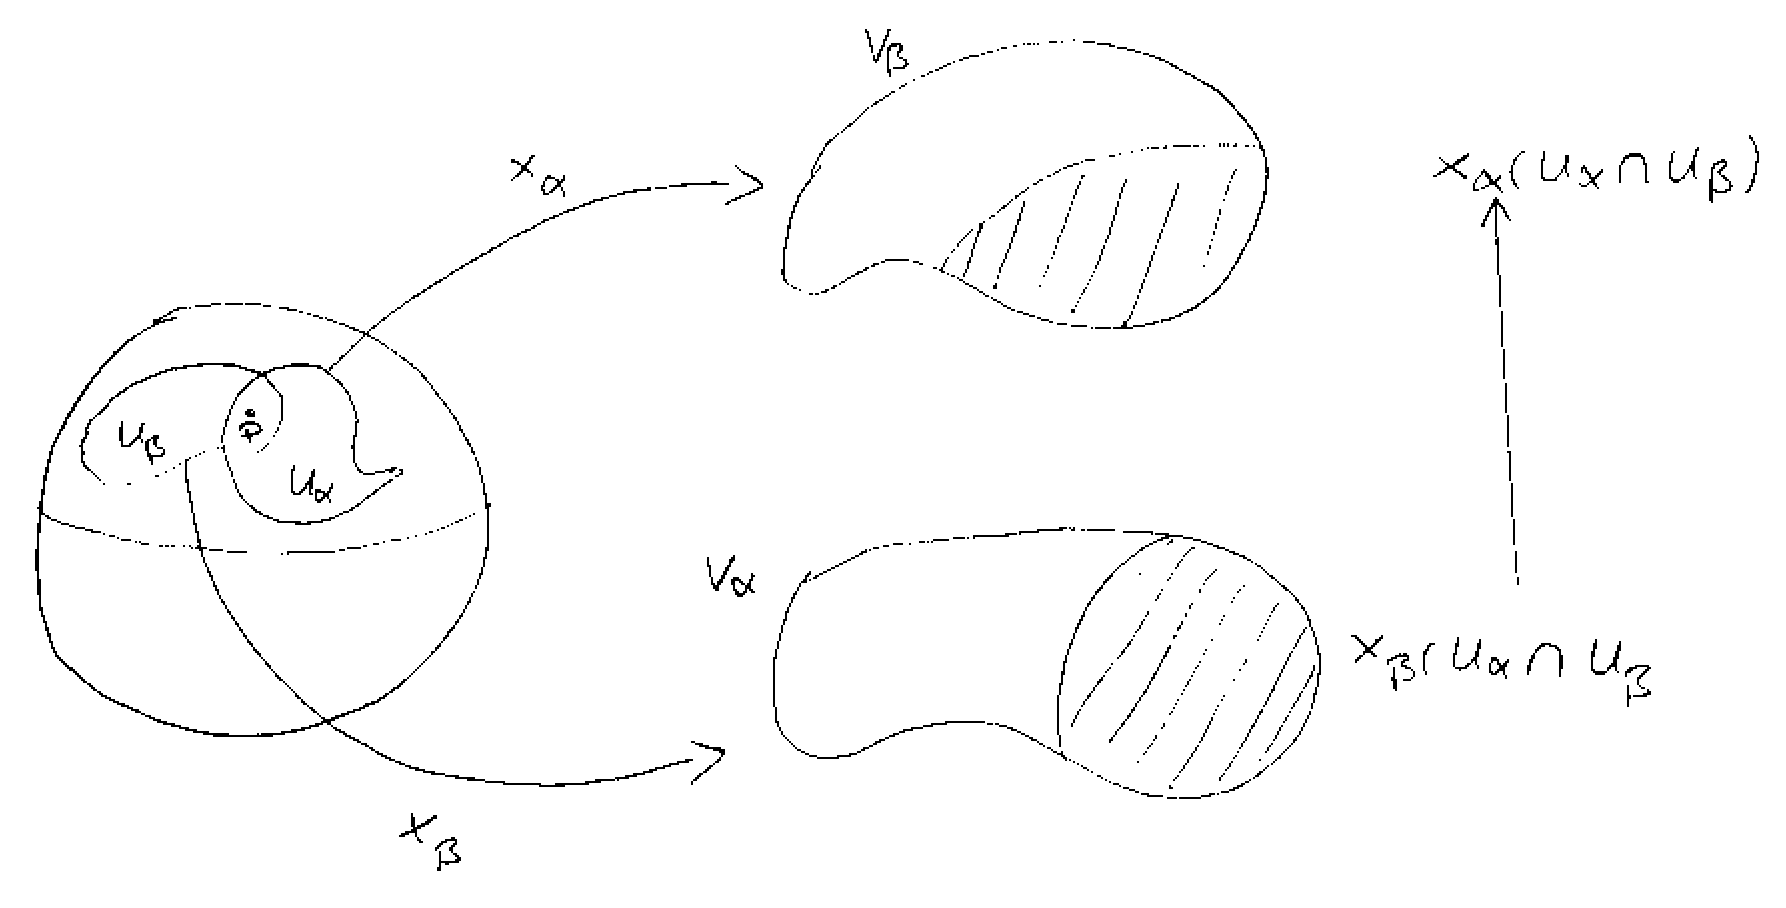
\includegraphics[width=0.8\linewidth]{figures/scan/kartenwechsel.png}
\caption{Kartenwechsel}
\label{img:kartenwechsel}
\end{figure} 

\end{defs}
Nun wollen wir, dass $x_{\alpha}\circ x_{\beta}^{-1}$ Diffeomorphismen sind.

\begin{defs}
Sei $ \mathcal{M}$ eine topologische Mannigfaltigkeit.
\begin{enumerate}
	\item[a)] Ein Atlas $\mathcal{A} = \{(x_{\alpha},U_{\alpha})\}$ auf $\mathcal{M}$ heißt $C^{\infty}$-Atlas, falls alle Kartenwechsel $x_{\alpha}\circ x_{\beta}^{-1}$ mit $\alpha, \beta \in A \ C^{\infty}$-Diffeomorphismen sind.
	\item[b)] Sei $\mathcal{A}$ ein $C^{\infty}$-Atlas von $\mathcal{M}$. \\
	Eine Karte $(x,U)$ ist verträglich mit $\mathcal{A}$, falls $x \circ x^{-1}$ ein $C^{\infty}$-Diffeomorphismus ist.
\end{enumerate}
\end{defs}
Gegeben ein $C^{\infty}$-Atlas, so kann man diesen zu einem \textit{maximalen} $C^{\infty}$-Atlas vervollständigen. Maximal bedeutet hierbei, dass der Atlas nicht strikt in einem anderen enthalten ist.


	% !TeX root = ..//diffgeo_main.tex
\begin{defs}[Differenzierbare Mannigfaltigkeit]
Eine \textit{differenzierbare Struktur} auf einer topologischen Mannigfaltigkeit M ist ein \textit{maximaler $C^\infty$-Atlas}. Eine \textit{differenzierbare Mannigfaltigkeit} ist eine topologische Mannigfaltigkeit mit einer differenzierbaren Struktur.
\end{defs}

\begin{bem}
Man kann auch eine topologische Mannigfaltigkeit definieren, ohne das 2. Abzählbarkeitsaxiom zu fordern.
\begin{description}
\item[Aber:] Dann bekommt man Mannigfaltigen mit ganz anderen Eigenschaften als diejenigen, die wir betrachten wollen.
\item[Wichtig:] Hausdorffsch + 2. Abzählbarkeitsaxiom $\Rightarrow$ parakompakt, d. h. jede offene Überdeckung hat eine lokale Verfeinerung.
\end{description}
$(V_j)$ heißt Verfeinerung von $(U_j)$, falls $\forall V_j \exists U_j$ mit $V_j \subseteq U_j$\\
Lokal endlich: $\forall p \in X\ \exists$ Umgebung $U$, die nur endlich viele $U_i$ trifft\\
Parakompakt $\Rightarrow \exists$ Partition der Eins f mit 
\begin{align*}
f_i: V_i \subseteq X \rightarrow [0, 1],\ \sum_{i \in I} f_i (x) = 1
\end{align*} 
\end{bem}

\begin{bsp}
Metrische Räume sind parakompakt.
\end{bsp}

\begin{bsp}[differenzierbare Mannigfaltigkeiten]
\begin{enumerate}
\item$\mathbb{R}^n$ mit Atlas $\mathcal{A} = \{(\operatorname{id}, \R^n)\}$
\item$V$ Vektorraum, $B$ Basis mit $B = \{v_1, \cdots, v_n\}$, Atlas $\mathcal{A} = \set{(\chi_B, V)}$
\begin{align*}
& \chi_B: V \rightarrow \R^n\\
& v = \sum^n_{i=1} a_i v_i \mapsto \sum_{i=1}^n a_i e_i
\end{align*}
wobei $(e_1, \cdots, e_n)$ die Standartbasis ist.
\item$M\subseteq \R^n,\ (\chi_U, U)$ mit $\chi_U = \operatorname{id}\vert_U,\ V \subseteq M^n,\ M$ differenzierbare Mannigfaltigkeit, $\mathcal{A} = \set{(\chi_X, U)}$ Atlas von $M$\\
$\mathcal{A}_V = \set{(\chi_V, U_V}$ wobei $(\chi_V, U_V) = (\chi_{U\cap V}, U\cap V)$
\item$M_1 = S^1,\ M_2 = \R,\ M_1\times M_2 =$ "unendlicher Zylinder"
\end{enumerate}
\hspace{.06\textwidth}
\begin{minipage}[H]{0.8\textwidth}
Seien $M_1^{n_1}, M_1^{n_2}$ differenzierbare Mannigfaltigkeiten, so ist $M_1\times M_2$ ebenfalls eine \difM \ der Dimension $n_1 + n_2$.\\
Atlas $\mathcal{A} = \set{(x\times y, U\times V)}$, wobei 
\begin{align*}
(x, U) &= \text{Karte von } M_1\\
(y, V) &= \text{Karte von } M_2
\end{align*}
$(x\times y)(p_1, p_2) = (x(p_1), y(p_2))$
\end{minipage}
\hspace{1cm}
\begin{minipage}[H]{.2\textwidth}
\vspace{-1.5cm}

\includegraphics[scale=0.5]{figures/tikz/cylinder.pdf}
\end{minipage}
\end{bsp}

\begin{bem}
$N$ mit der Teilraumtopologie und dem Atlas $\mathcal{A}_N = \set{(\chi\vert_U, U\cap N)}$ ist eine \difM.
\end{bem}

\begin{defs}
Seien $M, N$ differenzierbare Mannigfaltigkeiten. Eine \textit{Einbettung} ist eine differenzierbare Abbildung
\begin{align*}
f: N \rightarrow M
\end{align*}
sodass
\begin{enumerate}
\item$f(N)\subset M$ eine Untermannigfaltigkeit 
\item$f: N \rightarrow f(N)$ Diffeomorphismus
\end{enumerate}
\end{defs}

\section{Tangentialraum} 

\missingfigure{Tangentialräume}

\begin{defs}
\begin{enumerate}
\item Ein Tangentialvektor an $M$ im Punkt $p \in M$ ist eine $\R$-lineare Abbildung
\begin{align*}
v: \mathcal{F}(M) \rightarrow \R
\end{align*}
mit $v(fg) = v(f)g(p) + f(p)v(g)$.
\item Die Menge aller Tangentialvektoren an $M$ in $p$ heißt \textit{Tangentialraum} von $M$ in $p$: $T_pM$\\
$T_pM$ ist ein Vektorraum.
\end{enumerate}

\begin{figure}[h]
\centering
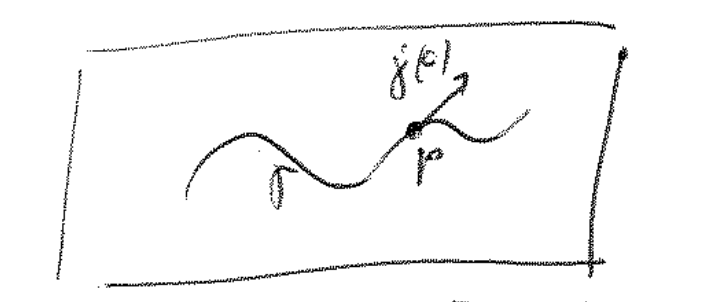
\includegraphics[width=0.5\linewidth]{figures/scan/tangentialvektorankurve.png}
\caption{Tangentialvektor an einer Kurve}
\label{img:tangentialvektorankurve}
\end{figure}

\end{defs}

	% !TeX root = ..//diffgeo_main.tex
\begin{hlem}[Existenz einer Glockenfunktion]
Sei $U \subseteq M$ offen, $p \in U$. Dann $\exists \varphi \in \mathcal{F}(M)$, s. d. 
\begin{enumerate}\label{Glockenfunktion}
\item$\operatorname{supp}\varphi\subseteq U$
\item$\varphi$ auf einer Umgebung $U' \subset U$ von $p$ ist
\end{enumerate}
\end{hlem}

\begin{figure}[H]
\centering 
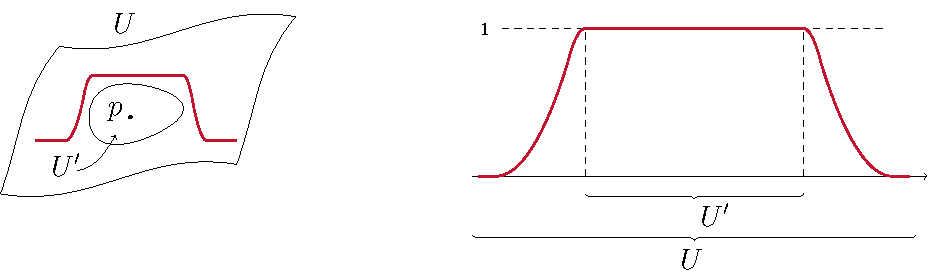
\includegraphics[scale=0.8]{figures/tikz/bump_function.pdf}
\caption{Visualisierung des Hilfslemmas  (\ref{Glockenfunktion}) \  ("bump function") }
\end{figure}

\begin{bew}
Sei $(x, U)$ eine Karte um $\varphi$, $\varepsilon > 0$, s. d. $B_{2\varepsilon}(x(p))\subset V\subset \R^n$ und wähle $\psi:\R^n\rightarrow\R$ mit 
\begin{align*}
\left.
\begin{array}{r}
\operatorname{supp}(\varphi)\subset B_{2\varepsilon}(x(p))\\
\varphi = 1 \text{ auf } B_\varepsilon
\end{array}
\right\} \text{ Resultat aus Analysis}\\
\end{align*}

Setze $\varphi(q) = \left\{
\begin{array}{l}
\psi(x(q))\text{ für }q\in U\\
0 \text{ sonst}
\end{array}
\right.$
\end{bew}

\begin{satz}[Eigenschaften des Tangentialraums]
Für $v\in T_p M$ gilt:
\begin{enumerate}
\item$v(\text{konstante Funktion}) = 0$
\item Falls $f = g$ in einer Umgebung von $p$, so gilt $v(f) = v(g)$
\end{enumerate}
"Lokalisierung von Tangentialvektoren"
\end{satz}

\begin{bew}[zu 2]
Wähle $\varphi$ wie im Hilfslemma, wobei $U$so gewählt ist, dass $\varphi f = \varphi g$ auf $U$ ist. Nun gilt:
\begin{align*}
v(\varphi f) &= v(\varphi)f(p) + \varphi(p)v(f)\\
&= v(\varphi)f(p) + v(f)\\
v(\varphi g) &= v(\varphi)g(p) + v(g)
\end{align*}
Dann folgt $v(\varphi f) = v(\varphi g) \Leftrightarrow v(f) = v(g)$.
\end{bew}

\begin{bew}[zu 1]
	$v(\lambda f) = \lambda v(f),\ \lambda \in \R,\ f\in \mathcal{F}(\R)$\\
	\textit{zz:} $v(\lambda) = 0$. Aufgrund von $v(\lambda) = \lambda v(1)$ genügt es zu zeigen, dess $v(1) = 0$. Dies folgt aus der Produktregel
	\begin{align*}
	v(1) = v(1*1) = 1v(1) + v(1)1 = 2v(1) \Rightarrow v(1) = 0
	\end{align*}
\end{bew}


%	\input{content/VL4-260418}
	\chapter{Vektorbündel}
\section{Tangentialbündel}
Wir wollen nun alle Tangentialräume einer Mannigfaltigkeit $\mfk$ gemeinsam betrachten.
\begin{align}
T\mfk = \bigcup_{p\in \mfk} T_{p}\mfk = \{ (p, V) \vert p \in \mfk, v \in T_{p}\mfk \} 
\end{align}
Wir wollen nun die Struktur einer differenzierbaren Mannigfaltigkeit. 
Das heißt wir müssen eine Topologie und eine $\cinf$-Struktur auf $T\mfk$ definieren.
\begin{align}
\pi: T\mfk &\to \mfk \\
(p,V) &\mapsto p
\end{align}
Sei $(x, U)$ eine Karte von $\mfk^m$. 
Dann definieren wir eine Karte $(\overline{x}, \overline{U})$ von $T\mfk$ wie folgt:
\begin{align}
&\overline{U} = \pi^{-1}(U) = \bigcup_{p\in\mfk} T_{p}\mfk \\
&\overline{x}: \overline{U} \to x(U) \times \R^m \subset \R^{2m} \\
&(p, V) \mapsto (x(p), \xi)
\end{align}

\begin{figure}[h]
\centering
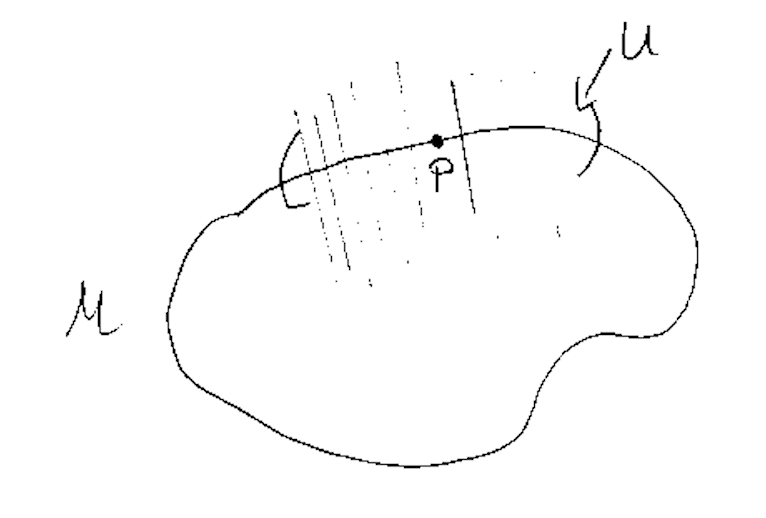
\includegraphics[width=0.4\linewidth]{figures/scan/tangentialbuendel.png}
\caption{Veranschaulichung eines Tangentialbündels}
\label{img:tangentialbuendel}
\end{figure} 

Wobei $\xi = (\xi^1, \dots, \xi^m) \in \R^m$ gegeben ist durch:
\begin{align}
v = \sum_{i=1}^{m} \xi_i \pdv{x_i} \big\vert_p, \quad \forall p \in U.
\end{align}
Wir haben noch keine Topologie auf $T\mfk$ definiert, das heißt $\overline{x}$ ist nur eine bijektive Abbildung zwischen Mengen.
Wir können allerdings nicht sagen ob es ein Homöomorphismus oder Diffeomorphismus ist.
Allerdings können wir Kartenwechsel betrachten.\\
Seien $(\overline{x}, \overline{U})$ und $(\overline{y}, \overline{U}')$ zwei Karten. 
Betrachte die Abbildungen:
\begin{align}
\overline{y} \circ \overline{x}^{-1} \circ \underbrace{x (\overline{U} \cap \overline{U}')}_{x(U \cap U') \times \R^m} \to \underbrace{\overline{y}(\overline{U} \cap \overline{U}')}_{y(U \cap U') \times \R^m}
\end{align}
\begin{align}
(x,\xi) \mapsto (y\circ x^{-1}(U), \eta) 
\end{align}
Wobei $\eta = \dd (y \circ x^{-1})\big\vert_U \xi$.\\
Da $y\circ x^{-1}$ Diffeomorphismus ist, ist $\overline{y} \circ \overline{x}^{-1}$ ein Isomorphimus.
Nun können wir die Topologie auf $T\mfk$ definieren.
$O \subset T\mfk$ offen, falls $\overline{x}(O\cap \overline{U})$ offen in $V \times \R^m$ ist für alle Karten $(x, U) \in \atlas_\mfk$ (bzw $(\overline{x}, \overline{U}) \in \atlas_{T\mfk}$)
\begin{satz}
$T\mfk$ mit dieser Topologie ist eine topologische Mannigfaltigkeit und $\atlas_{T\mfk}$ eine differenzierbare Struktur.
\end{satz}
\section{Vektorbündel}
$T\mfk$ hat die Struktur einer glatten Mannigfaltigkeit.
Allerdings hat es noch mehr, nämchlich die eines Vektorbündels, was wir nun definieren.
\begin{defs}[Vektorbündel]
Sei $\mfk$ eine differenzierbare Mannigfaltigkeit.
Ein $\R$-Vektorbündel vom $\rang$ $k$ über $\mfk$ ist eine differenzierbare Mannigfaltigkeit mit einer glatten surjektiven Abbildung:
\begin{align}
\pi: E \to \mfk,
\end{align}
so dass:
\begin{enumerate}
\item $\forall p \in \mfk$ hat $E_p:= \pi^{-1}( \{ p \})$ die Struktur eines $\R$-Vektorraums der Dimension $k$.
$E_p$ heißt Faser von $E$ über $p$.
\item Für alle $p$ in $\mfk$ existiert eine Umgebung $U$ von $p$ in $\mfk$ und ein Diffeomorphismus.
\begin{align}
\begin{xy}
\xymatrix@=0.2\linewidth{
      \phi: U \times \R^k \ar[rr] \ar[rd]_{pr_1}  &     &  \pi^{-1}(U) \ar[dl]^{\pi}  \\
                             &  U  &}
\end{xy}
\end{align}
%\begin{figure}[h]
%\centering
%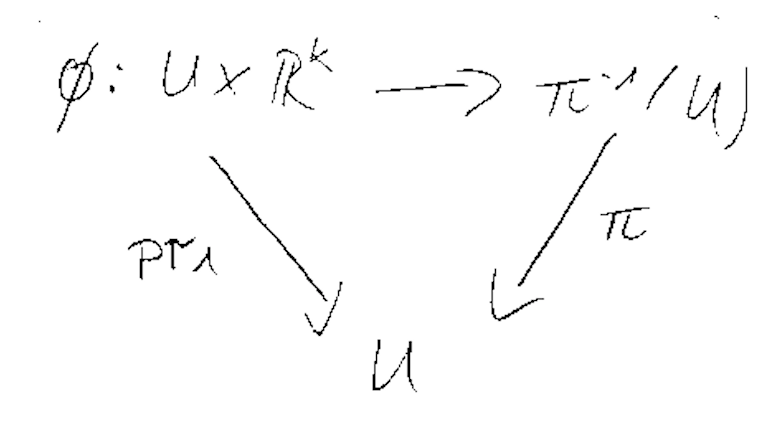
\includegraphics[width=0.4\linewidth]{figures/scan/lokaletrivialisierung.png}
%\caption{Lokale Trivialisierung}
%\label{img:lokaletrivialisierung}
%\end{figure} 
Für diesen gilt:
\begin{itemize}
\item $\pi \circ \phi = p r_1$
\item Für alle $q \in U$ ist die Abbildung
\begin{align}
\phi\big\vert_q : \{ q \} \times \R^k &\to E_q\\
\{ q, \xi \} &\mapsto \phi_q (\xi) := \phi(q, \xi)
\end{align}
$\phi$ heißt lokale Trivialisierung von $E$.
\end{itemize}
\end{enumerate}
\end{defs}
\begin{bem}
Ein Vektorbündel ist ein Tripel $(\pi, E, \mfk)$ aber wir schreiben oft nur $E$. Hierbei wird $E$ Totalraum und $\mfk$ Basis genannt.
\end{bem}
\begin{bsp} \leavevmode
\begin{enumerate}
\item Triviale Bündel:
\begin{align}
&E = \mfka \times \R^k \to \mfk\\
&(p, \xi) \mapsto p
\end{align}
\item Tangentialbündel 
\begin{align}
&\pi: T\mfk \to \mfk\\
&(p, V) \to V
\end{align}
\item Tautologisches Bündel
\begin{align}
&\mfk = \R \mathbb{P}^n\\
&E = \{ (l, x) \vert l \in \R \mathbb{P}^n, x\in l \subset \R^{n+1} \}\\
&\pi: E \to \mfk = \R \mathbb{P}^n\\
&(l, x) \mapsto l
\end{align}
Behauptung: Dies ist ein Vektorbündel vom $\rang$ $1$.
Vektorraumstruktur auf $E_l$:
\begin{align}
(l, x) + (l, y) &:= (l, x + y)\\
k (l, x) &:= (l, k x)
\end{align}
\end{enumerate}
\end{bsp}
Nun wollen wir uns damit beschäftigen wie wir Vektorbündel konstruieren können.
Angenommen uns wäre das folgende gegeben:
\begin{enumerate}
\item $E_p, p\in \mfk$ eine Familie von Vektorräumen der Dimension $k$
\item $(U_\alpha)_{\alpha \in \atlas}$ eine offene Überdeckung von $\mfk$
\item $\forall \alpha \in \atlas$, $p\in U_\alpha$ gibt es den folgenden Isomorphismus:
\begin{align}
\phi_{\alpha, p}: \R^\alpha \to E_p
\end{align}
\end{enumerate}
Setze 
\begin{align}
&E = \cup_{p \in \mfk} E_p\\
&\pi : E \to \mfk\\
&(p, V) \mapsto p\\
&\phi_\alpha: U_\alpha \times \R^k \to E \big\vert_{U_\alpha}\\
&(p, \xi) \mapsto (p, \phi_{\alpha, p}(\xi)).
\end{align}
Nun stellt sich die Frage unter welchen Vorraussetzungen $(\pi, E, \mfk)$ ein Vektorbündel ist.
\begin{lem}
\label{lem:vorraussetzungenvektorbündel}
Sei $\mfk$ eine glatte Mannigfaltigkeit, $E$ eine Menge und die Abbildung $\pi: E\to\mfk$ surjektiv.
Sei $\{ U_\alpha \}$ eine offene Überdeckung von $\mfk$ zusammen mit bijektiven Abbildungen
\begin{align}
\phi^{-1}_{\alpha} = \varphi: \pi^{-1}(U_\alpha) \to U_\alpha \times \R^\alpha,
\end{align}
die $pr_1 \circ \varphi_\alpha = \pi$ erfüllen, so dass wann immer $U_\alpha \cap U_\beta \neq \emptyset$, dann ist 
\begin{align}
\varphi_\alpha \circ \varphi_{\beta}^{-1} \to (U_\alpha \cap U_\beta) \times \R^k,
\end{align}
von der Form:
\begin{align}
\label{eq:konstruktionvektorbündel}
(\varphi_\alpha \circ \varphi_{\beta}^{-1})(p, v) = (p, \tau(p) v)
\end{align}
mit einer glatten Abbildung $\tau: U_\alpha \cap U_\beta \to \mathrm{GL}(k, \R)$.
Dann existiert eine eindeutige Struktur als glattes $k$-dim Vektorbündel über $\mfk$ für die $\varphi^{-1}_{\alpha}$ lokale Trivialisierungen sind.
\end{lem}
\begin{bew}[Beweis Lemma \ref{lem:vorraussetzungenvektorbündel}]
Sei  $p\in\mfk$. 
Setze $E_p := \pi^{-1}(\{ p \})$. 
Falls $p\in U_\alpha$, dann ist 
\begin{align}
\varphi_\alpha \big\vert_p : E_p \to \{ p \} \times \R^k.
\end{align}
Definiere eine Vektorraumstruktur auf $E_p$ durch die Forderung, dass die Abbildung $\varphi_\alpha \big\vert_p$ ein Isomorphismus ist.
Durch verkleinern von $U_\alpha$ und hinzunahme von weiteren offenen Mengen kann man annehmen, dass jedes $U_\alpha$ diffeomorph zu $\overline{U}_\alpha \subseteq \R^m$ ist.
Verknüpfung von $\varphi_\alpha$ mit einem solchen Diffeomorphismus liefert eine Bijektion:
\begin{align}
\pi^{-1} (U_\alpha) \to \overline{U}_\alpha \times \R^k .
\end{align}
Diese nutzen wir als Karte für $E$.
Wegen Gleichung \ref{eq:konstruktionvektorbündel} bekommen wir eine glatte Struktur auf $E$.
\end{bew}
Sei $(x, U)$ Karte von $\mfk$, $p\in U$, $v\in T_p \mfk$.
\begin{align}
v = \sum_{i=1}^{m} \xi_i \pdv{x_i}\big\vert_p
\end{align}
Definiere:
\begin{align}
\varphi: \pi^{-1} (U) &\to U \times \R^m\\
v &\mapsto (p, V)
\end{align}
Dort wo $(x)$ und $(\overline{x})$ überlappen.
\begin{align}
\pdv{x_i} \big\vert_p &= (\pdv{\overline{x}_j}{x_i})\pdv{\overline{x}_j} \big\vert\\
v &= \sum_{j=1}^{m} \xi_j \pdv{\overline{x}_j}  \big\vert_p = \sum_{ji1}^{m} \xi_i \pdv{\overline{x}_i}  \big\vert_p \\
&= \sum_{i, j}^{m} \xi_i \pdv{\overline{x}_j}{x_i}  \pdv{\overline{x}_j}\big\vert_p\\
&\Rightarrow \overline{\xi}_j = \sum_i v_i \pdv{\overline{x}_j}{x_i}
\end{align}
\begin{align}
\varphi \circ \varphi^{-1}(x, v) = (x, \overline{v}) = (x, \tau(x), v)
\end{align}
Wobei nun $\tau(x)$ gegeben ist durch $\pdv{\overline{x}_j}{x_i}$
	% !TeX root = ..//diffgeo_main.tex
\chapter{Vektorbündel}
\section{Tangentialbündel}
Wir wollen nun alle Tangentialräume einer Mannigfaltigkeit $\mfk$ gemeinsam betrachten.
\begin{align}
T\mfk = \bigcup_{p\in \mfk} T_{p}\mfk = \{ (p, V) \vert p \in \mfk, v \in T_{p}\mfk \} 
\end{align}
Wir wollen nun die Struktur einer differenzierbaren Mannigfaltigkeit. 
Das heißt wir müssen eine Topologie und eine $\cinf$-Struktur auf $T\mfk$ definieren.
\begin{align}
\pi: T\mfk &\to \mfk \\
(p,V) &\mapsto p
\end{align}
Sei $(x, U)$ eine Karte von $\mfk^m$. 
Dann definieren wir eine Karte $(\overline{x}, \overline{U})$ von $T\mfk$ wie folgt:
\begin{align}
&\overline{U} = \pi^{-1}(U) = \bigcup_{p\in\mfk} T_{p}\mfk \\
&\overline{x}: \overline{U} \to x(U) \times \R^m \subset \R^{2m} \\
&(p, V) \mapsto (x(p), \xi)
\end{align}

\begin{figure}[h]
\centering
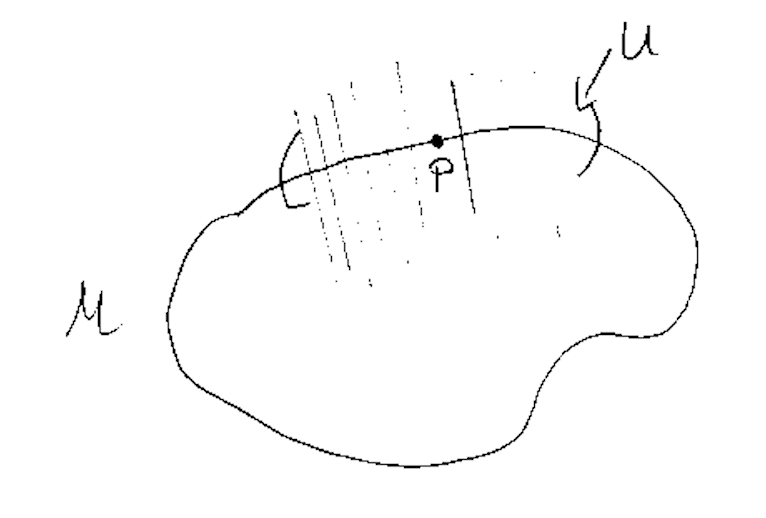
\includegraphics[width=0.4\linewidth]{figures/scan/tangentialbuendel.png}
\caption{Veranschaulichung eines Tangentialbündels}
\label{img:tangentialbuendel}
\end{figure} 

Wobei $\xi = (\xi^1, \dots, \xi^m) \in \R^m$ gegeben ist durch:
\begin{align}
v = \sum_{i=1}^{m} \xi_i \pdv{x_i} \big\vert_p, \quad \forall p \in U.
\end{align}
Wir haben noch keine Topologie auf $T\mfk$ definiert, das heißt $\overline{x}$ ist nur eine bijektive Abbildung zwischen Mengen.
Wir können allerdings nicht sagen ob es ein Homöomorphismus oder Diffeomorphismus ist.
Allerdings können wir Kartenwechsel betrachten.\\
Seien $(\overline{x}, \overline{U})$ und $(\overline{y}, \overline{U}')$ zwei Karten. 
Betrachte die Abbildungen:
\begin{align}
\overline{y} \circ \overline{x}^{-1} \circ \underbrace{x (\overline{U} \cap \overline{U}')}_{x(U \cap U') \times \R^m} \to \underbrace{\overline{y}(\overline{U} \cap \overline{U}')}_{y(U \cap U') \times \R^m}
\end{align}
\begin{align}
(x,\xi) \mapsto (y\circ x^{-1}(U), \eta) 
\end{align}
Wobei $\eta = \dd (y \circ x^{-1})\big\vert_U \xi$.\\
Da $y\circ x^{-1}$ Diffeomorphismus ist, ist $\overline{y} \circ \overline{x}^{-1}$ ein Isomorphimus.
Nun können wir die Topologie auf $T\mfk$ definieren.
$O \subset T\mfk$ offen, falls $\overline{x}(O\cap \overline{U})$ offen in $V \times \R^m$ ist für alle Karten $(x, U) \in \atlas_\mfk$ (bzw $(\overline{x}, \overline{U}) \in \atlas_{T\mfk}$)
\begin{satz}
$T\mfk$ mit dieser Topologie ist eine topologische Mannigfaltigkeit und $\atlas_{T\mfk}$ eine differenzierbare Struktur.
\end{satz}
\section{Vektorbündel}
$T\mfk$ hat die Struktur einer glatten Mannigfaltigkeit.
Allerdings hat es noch mehr, nämchlich die eines Vektorbündels, was wir nun definieren.
\begin{defs}[Vektorbündel]
Sei $\mfk$ eine differenzierbare Mannigfaltigkeit.
Ein $\R$-Vektorbündel vom $\rang$ $k$ über $\mfk$ ist eine differenzierbare Mannigfaltigkeit mit einer glatten surjektiven Abbildung:
\begin{align}
\pi: E \to \mfk,
\end{align}
so dass:
\begin{enumerate}
\item $\forall p \in \mfk$ hat $E_p:= \pi^{-1}( \{ p \})$ die Struktur eines $\R$-Vektorraums der Dimension $k$.
$E_p$ heißt Faser von $E$ über $p$.
\item Für alle $p$ in $\mfk$ existiert eine Umgebung $U$ von $p$ in $\mfk$ und ein Diffeomorphismus.
\begin{align}
\begin{xy}
\xymatrix@=0.2\linewidth{
      \phi: U \times \R^k \ar[rr] \ar[rd]_{pr_1}  &     &  \pi^{-1}(U) \ar[dl]^{\pi}  \\
                             &  U  &}
\end{xy}
\end{align}
%\begin{figure}[h]
%\centering
%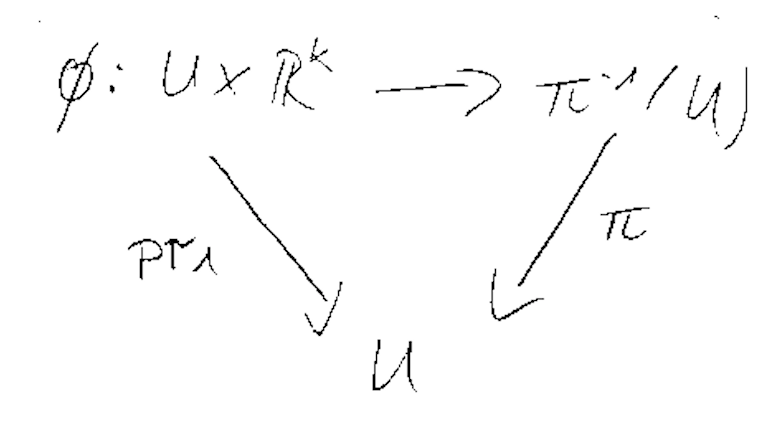
\includegraphics[width=0.4\linewidth]{figures/scan/lokaletrivialisierung.png}
%\caption{Lokale Trivialisierung}
%\label{img:lokaletrivialisierung}
%\end{figure} 
Für diesen gilt:
\begin{itemize}
\item $\pi \circ \phi = p r_1$
\item Für alle $q \in U$ ist die Abbildung
\begin{align}
\phi\big\vert_q : \{ q \} \times \R^k &\to E_q\\
\{ q, \xi \} &\mapsto \phi_q (\xi) := \phi(q, \xi)
\end{align}
$\phi$ heißt lokale Trivialisierung von $E$.
\end{itemize}
\end{enumerate}
\end{defs}
\begin{bem}
Ein Vektorbündel ist ein Tripel $(\pi, E, \mfk)$ aber wir schreiben oft nur $E$. Hierbei wird $E$ Totalraum und $\mfk$ Basis genannt.
\end{bem}
\begin{bsp} \leavevmode
\begin{enumerate}
\item Triviale Bündel:
\begin{align}
&E = \mfka \times \R^k \to \mfk\\
&(p, \xi) \mapsto p
\end{align}
\item Tangentialbündel 
\begin{align}
&\pi: T\mfk \to \mfk\\
&(p, V) \to V
\end{align}
\item Tautologisches Bündel
\begin{align}
&\mfk = \R \mathbb{P}^n\\
&E = \{ (l, x) \vert l \in \R \mathbb{P}^n, x\in l \subset \R^{n+1} \}\\
&\pi: E \to \mfk = \R \mathbb{P}^n\\
&(l, x) \mapsto l
\end{align}
Behauptung: Dies ist ein Vektorbündel vom $\rang$ $1$.
Vektorraumstruktur auf $E_l$:
\begin{align}
(l, x) + (l, y) &:= (l, x + y)\\
k (l, x) &:= (l, k x)
\end{align}
\end{enumerate}
\end{bsp}
Nun wollen wir uns damit beschäftigen wie wir Vektorbündel konstruieren können.
Angenommen uns wäre das folgende gegeben:
\begin{enumerate}
\item $E_p, p\in \mfk$ eine Familie von Vektorräumen der Dimension $k$
\item $(U_\alpha)_{\alpha \in \atlas}$ eine offene Überdeckung von $\mfk$
\item $\forall \alpha \in \atlas$, $p\in U_\alpha$ gibt es den folgenden Isomorphismus:
\begin{align}
\phi_{\alpha, p}: \R^\alpha \to E_p
\end{align}
\end{enumerate}
Setze 
\begin{align}
&E = \cup_{p \in \mfk} E_p\\
&\pi : E \to \mfk\\
&(p, V) \mapsto p\\
&\phi_\alpha: U_\alpha \times \R^k \to E \big\vert_{U_\alpha}\\
&(p, \xi) \mapsto (p, \phi_{\alpha, p}(\xi)).
\end{align}
Nun stellt sich die Frage unter welchen Vorraussetzungen $(\pi, E, \mfk)$ ein Vektorbündel ist.
\begin{lem}
\label{lem:vorraussetzungenvektorbündel}
Sei $\mfk$ eine glatte Mannigfaltigkeit, $E$ eine Menge und die Abbildung $\pi: E\to\mfk$ surjektiv.
Sei $\{ U_\alpha \}$ eine offene Überdeckung von $\mfk$ zusammen mit bijektiven Abbildungen
\begin{align}
\phi^{-1}_{\alpha} = \varphi: \pi^{-1}(U_\alpha) \to U_\alpha \times \R^\alpha,
\end{align}
die $pr_1 \circ \varphi_\alpha = \pi$ erfüllen, so dass wann immer $U_\alpha \cap U_\beta \neq \emptyset$, dann ist 
\begin{align}
\varphi_\alpha \circ \varphi_{\beta}^{-1} \to (U_\alpha \cap U_\beta) \times \R^k,
\end{align}
von der Form:
\begin{align}
\label{eq:konstruktionvektorbündel}
(\varphi_\alpha \circ \varphi_{\beta}^{-1})(p, v) = (p, \tau(p) v)
\end{align}
mit einer glatten Abbildung $\tau: U_\alpha \cap U_\beta \to \mathrm{GL}(k, \R)$.
Dann existiert eine eindeutige Struktur als glattes $k$-dim Vektorbündel über $\mfk$ für die $\varphi^{-1}_{\alpha}$ lokale Trivialisierungen sind.
\end{lem}
\begin{bew}[Beweis Lemma \ref{lem:vorraussetzungenvektorbündel}]
Sei  $p\in\mfk$. 
Setze $E_p := \pi^{-1}(\{ p \})$. 
Falls $p\in U_\alpha$, dann ist 
\begin{align}
\varphi_\alpha \big\vert_p : E_p \to \{ p \} \times \R^k.
\end{align}
Definiere eine Vektorraumstruktur auf $E_p$ durch die Forderung, dass die Abbildung $\varphi_\alpha \big\vert_p$ ein Isomorphismus ist.
Durch verkleinern von $U_\alpha$ und hinzunahme von weiteren offenen Mengen kann man annehmen, dass jedes $U_\alpha$ diffeomorph zu $\overline{U}_\alpha \subseteq \R^m$ ist.
Verknüpfung von $\varphi_\alpha$ mit einem solchen Diffeomorphismus liefert eine Bijektion:
\begin{align}
\pi^{-1} (U_\alpha) \to \overline{U}_\alpha \times \R^k .
\end{align}
Diese nutzen wir als Karte für $E$.
Wegen Gleichung \ref{eq:konstruktionvektorbündel} bekommen wir eine glatte Struktur auf $E$.
\end{bew}
Sei $(x, U)$ Karte von $\mfk$, $p\in U$, $v\in T_p \mfk$.
\begin{align}
v = \sum_{i=1}^{m} \xi_i \pdv{x_i}\big\vert_p
\end{align}
Definiere:
\begin{align}
\varphi: \pi^{-1} (U) &\to U \times \R^m\\
v &\mapsto (p, V)
\end{align}
Dort wo $(x)$ und $(\overline{x})$ überlappen.
\begin{align}
\pdv{x_i} \big\vert_p &= (\pdv{\overline{x}_j}{x_i})\pdv{\overline{x}_j} \big\vert\\
v &= \sum_{j=1}^{m} \xi_j \pdv{\overline{x}_j}  \big\vert_p = \sum_{ji1}^{m} \xi_i \pdv{\overline{x}_i}  \big\vert_p \\
&= \sum_{i, j}^{m} \xi_i \pdv{\overline{x}_j}{x_i}  \pdv{\overline{x}_j}\big\vert_p\\
&\Rightarrow \overline{\xi}_j = \sum_i v_i \pdv{\overline{x}_j}{x_i}
\end{align}
\begin{align}
\varphi \circ \varphi^{-1}(x, v) = (x, \overline{v}) = (x, \tau(x), v)
\end{align}
Wobei nun $\tau(x)$ gegeben ist durch $\pdv{\overline{x}_j}{x_i}$
	% !TeX root = ..//diffgeo_main.tex
Im Folgenden werden nun einige Beispiele für Vektorbündel angeben.
\subsection{Direkte Summe (Whitney-Summe)}
Es seien zwei Vektorbündel gegeben:
\begin{align}
\pi : E &\to \mfk \\
\pi ' : E' & \to \mfk '
\end{align}
mit $\rang$ $k$ bzw. $k'$. 
Dann existiert $(U_\alpha)_{\alpha \in A}$ eine offene Überdeckung, sodass für alle $\alpha \in A$ und alle $p \in U_\alpha$ folgendes gilt:
\begin{align}
&\phi_{\alpha, p}: \R^k \to E_p, \quad g_{\alpha, \beta}: U_\alpha \cap U_\beta \to \mathrm{Gl}(k, \R)\\
&\phi_{\alpha, p}': \R^{k'} \to E_{p}', \quad g_{\alpha, \beta}': U_\alpha \cap U_\beta \to \mathrm{Gl}(k', \R)
\end{align}  
Wir definieren:
\begin{align}
&\mathcal{E}_p := E_p \oplus E_{p}\\
&\mathcal{E} = \bigcup_{p \in \mfk} \mathcal{E}_p
\end{align}
\begin{align}
&\Phi_{\alpha, p}: \R^k \oplus \R^{k'} \to E_P \oplus E_{p}'\\
&(v, w) \mapsto (\phi_{\alpha \ p} (v), \phi_{\alpha \ p}' (w))
\end{align}
\begin{align}
&G_{\alpha \beta}: U_\alpha \cap U_\beta \to \mathrm{Gl}(k + k', \R)\\
&p \mapsto \begin{pmatrix}
g_{\alpha \beta}(p)  & 0 \\ 
0  & g_{\alpha \beta}'(p)
\end{pmatrix} 
\end{align}
$\mathcal{E}$ ist nun ein Vektorbündel. 
Wir nennen $\mathcal{E}$ die Whitney-Summe von $E$ und $E'$ und schreiben:
\begin{align}
\mathcal{E} = E \oplus E'.
\end{align} 

\subsection{Tensorbündel}
Es seien $E'$ und $E''$ Vektorbündel über $\mfk$ und $(U_\alpha)$ sei wie oben definiert.
\begin{align}
(E' \oplus E'')_p &:= E_{p}'\oplus E_{p}''\\
\phi_{\alpha \ p} : \R^{k'} \times \R^{k''} &\to E_{p}' \oplus E_{p}''\\
(v, w) &\mapsto \phi_{\alpha \ p}'(v) \oplus \phi_{\alpha \ p}'' (w)
\end{align}
Wir erhalten zusammen die Folgende Übergangsmatrix:
\begin{align}
g_{\alpha \beta} = g_{\alpha \beta}'(p) \oplus g_{\alpha \beta}''(p)
\end{align}
Diese Abbildung ist glatt und somit ergibt sich somit ein neues Vektorbündel.

\subsection{Homomorphismenbündel}
Es seien die Daten wie eben schon gegeben.
Das Homomorphismenbündel
\begin{align}
\mathrm{Hom}_p := \mathrm{Hom}(E_{p}', E_{p}'')
\end{align}
ist wie folgt gegeben:
\begin{align}
\phi_{\alpha \ p} : \mathrm{Hom}(\R^{k'}, \R^{k''}) &\to \mathrm{Hom}(E_{p}', E_{p}'')\\
f &\mapsto \phi_{\alpha \ p} \circ f \circ (\phi_{\alpha \ p}')^{-1}
\end{align}

\subsection{Duales Bündel}
Sei ein Vektorbündel $(\pi, E, \mfk)$ gegeben. 
Wir wollen nun das sogenannte duale Vektorbündel konstruieren.
Hierbei führen wir folgende Notation ein $E^* = \mathrm{Hom}(E, \R)$.
Hierbei ist $\R$ das triviale Vektorbündel vom Rang $1$.
Ein wichtiges Beispiel ist hierbei das Kotangentialbündel $T^{*}\mfk = \mathrm{Hom}(T\mfk , \R)$.
$T^{*}_{p}\mfk$ heißt der Kotangentialraum.\\
Sei $f: \mfk \to \R$ eine glatte Abbildung.
\begin{align}
\dd f \big\vert_p : T_p \mfk \to T_{f(p)}\R \cong \R
\end{align}
Es gilt $\dd f\big\vert_p \in T_p^* \mfk \subset T^* \mfk$.
Sei $x: U \to x(U)$ eine Karte 
\begin{align}
\dd x \big\vert_p : T_p \mfk \to \rn
\end{align}
Die so definierten Differentiale $\{ \dd x^1 \big\vert_p, \dots , \dd x^n \big\vert_p \}$ bilden eine Basis für $T_p^* \mfk$.
\begin{itemize}
\item $\dd x^i \big\vert_p$ heißen Kotangentialvektoren
\item $\pdv{x^i} \big\vert_p$ heißen Tangentialvektoren
\end{itemize}
Seien $(x, U)$ und $(y, U')$ zwei Karten um p.
\begin{align}
\pdv{x^i}\big\vert_p &= \sum_j a^j_i \pdv{y^j} \big\vert_p, \quad a^j_i = \pdv{y^j}{x^i} \\
\dd x^k &= \sum b^k_l \dd y^l \big\vert_p = \sum \pdv{x^k}{y^l} \dd y^l \big\vert_p
\end{align}

\subsection{Alternierendes Vektorbündel}
Das Alternierende Vektorbündel
\begin{align}
\wedge^m(E', E'')_p &:= \wedge^m(E_{p}', E_{p}'')\\
&= \{ f: \underbrace{E_{p}' \times \dots \times E_{p}'}_{n-\mathrm{mal}} \to E_{p}'' \}
\end{align}
Wobei $f$ multilinear und alternierend ist. 
\begin{align}
&\phi_{\alpha \ p}: \wedge^n (\R^{k'}, \R^{k''}) \to \wedge^n (E_{p}', E_{p}'')\\
&f \mapsto ((v_1, \dots, v_n) \mapsto \phi_{\alpha p}''( f(\phi_{\alpha p})^{-1} (v_1), \dots f(\phi_{\alpha p})^{-1} (v_n)) )
\end{align}
Es bleibt zu zeigen, dass $g_{\alpha \beta}$ glatt ist.\\
Es gilt 
\begin{align}
\wedge^1 (E', E'') &= \mathrm{Hom}(E', E'')\\
\wedge^1 (T\mfk, \R) &= T^{*}\mfk
\end{align}

\begin{defs}[Bündel-Abbildung]
Seien $(\pi, E, \mfk)$ und $(\pi, E', \mfk')$ Vektorbündel.
Ein paar $(f, L)$ von glatten Abbildungen $f: \mfk \to \mfk'$ und $L: E \to E'$ heißt Bündelabbildung falls:
\begin{itemize}
\item $\pi' \circ L = f \circ \pi$
\item $L\big\vert_{E_p}$ ist $\R$-linear
\end{itemize}


\begin{align}
\begin{xy}
  \xymatrix@=0.25\linewidth{
      E \ar[r]^L \ar[d]_\pi    &   E' \ar[d]^{\pi '}  \\
      \mfk \ar[r]_f             &   \mfk'   
  }
\end{xy}
\end{align}
%\begin{figure}[h]
%\centering
%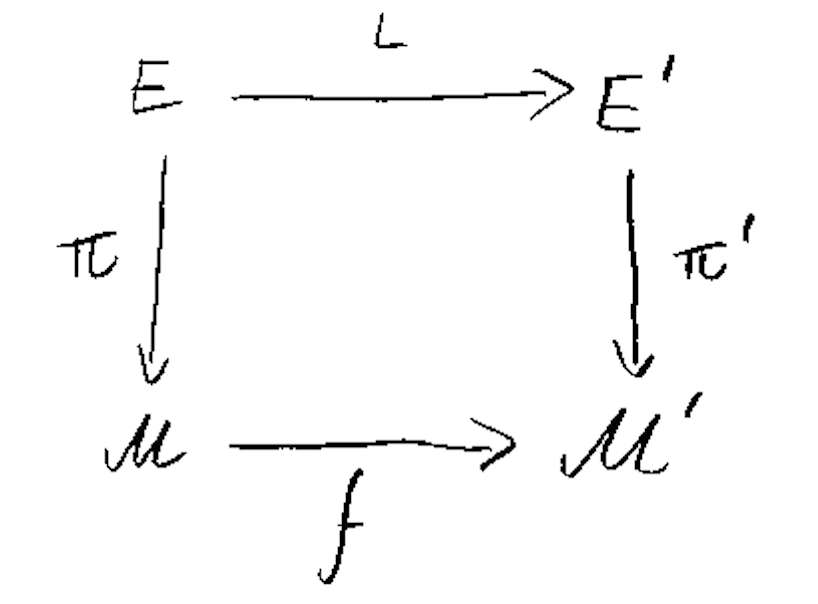
\includegraphics[width=0.4\linewidth]{figures/scan/buendelabbildung.png}
%\label{img:buendelabbildung}
%\end{figure} 


\end{defs}

\begin{bsp}
Seien $\mfk$,$\mfk'$ glatte Mannigfaltigkeiten und $f:\mfk \to \mfk'$ glatt.
Dann ist $(f, \dd f)$ eine Bündel-Abbildung von $T\mfk$ nach $T\mfk'$.
\end{bsp}

\begin{defs}[Unterbündel]
Sei $(\pi, E, \mfk)$ ein Vektorbündel mit Rang $k$.
Eine Untermannigfaltigkeit $E' \subset E$ ist ein Unterbündel vom Rang $k'$ falls
\begin{align}
\pi \big\vert_{E'}: E' \to \mfk,
\end{align}
Ein Vektorbündel ist.
\end{defs}

\begin{bsp}[Unterbündel] \leavevmode
\begin{enumerate}
\item $S^n \subset \R^{n+1}$
\begin{align}
TS^m \cong \{ (p,x)\in S^n \times \R^{n+1} \vert x \perp p \} \subset \underbrace{S^n \times \R^{n+1}}_{\mathrm{triviales} \ \mathrm{Bündel}}
\end{align}
ist ein Unterbündel
\item $\R \mathbb{P}^n$ mit dem tautologischen Bündel 
\begin{align}
\{ (l, x) \in \R \mathbb{P}^n \times \R^{n+1} \vert x \in l \} \subset \R\mathbb{P}^n \times \R^{n+1}
\end{align}
ist ein Unterbündel.
\end{enumerate}
\end{bsp}
\begin{defs}[Schnitte von Vektorbündeln]
Sei $(\pi, E, \mfk)$ ein Vektorbündel.
Eine glatte Abbildung $S:\mfk \to E$ heißt Schnitt von $E$, falls $\pi \circ s = \id\big\vert_{\mfk}$.
Wir bezeichnen die Schnitte von $E$ mit $\Gamma (E)$.\\
Sei $U \subset \mfk$. 
Ein Schnitt von $E$ über $U$ ist eine Abbildung $s : U \to E$ mit $\pi \circ s = \id_U$.
\end{defs}
\begin{bsp}[Schnitte] \leavevmode
\begin{itemize}
\item Nullschnitt
\begin{align}
&S : \mfk \to E \\
&p \mapsto 0 \in E_p
\end{align}
\item Schnitte von $T\mfk$ heißen Vektorfelder.
Wir bezeichnen die Vektorfelder $V: \mfk \to T\mfk$ mit $\mathfrak{X}(\mfk)$.

\begin{figure}[h]
\centering
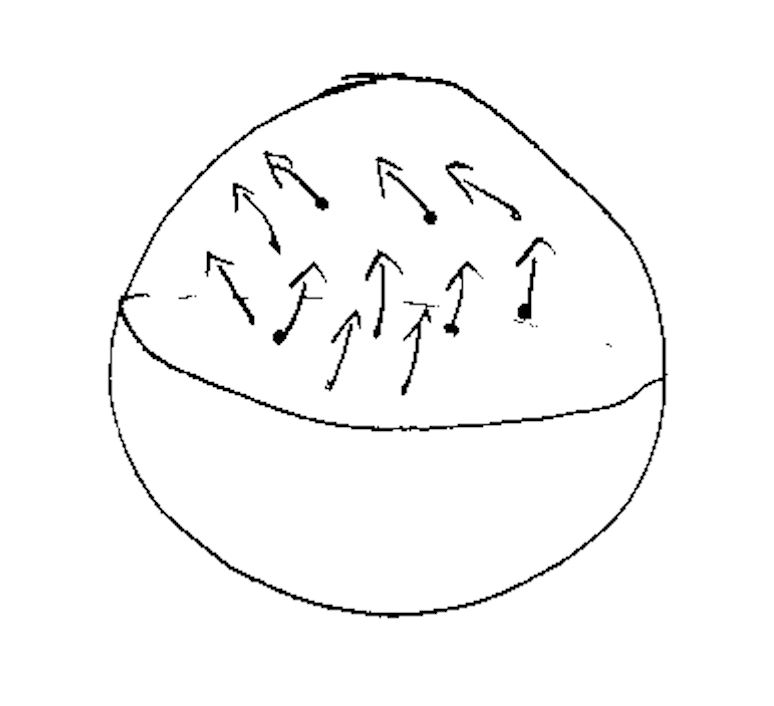
\includegraphics[width=0.4\linewidth]{figures/scan/bspvektorfeld.png}
\caption{Beispiel für ein Vektorfeld}
\label{img:bspvektorfeld}
\end{figure} 

\end{itemize}
\end{bsp}


\begin{satz}
\label{satz:SchnitteModul}
Der Raum der Schnitte $\Gamma (E)$ ist ein Modul über $\mathcal{F}(\mfk)$.
\end{satz}

\begin{bew}[Beweis Satz \ref{satz:SchnitteModul}]
Seien $s_1, s_2 \in \Gamma (E)$, so ist $s_1 + s_2 \in \Gamma (E)$
\begin{align}
(s_1 + s_2)(p) := s_1 (p) p s_2 (p)
\end{align}
Sei $\phi \in \mathcal{F}(\mfk), s\in \Gamma(E)$, so ist $\phi \circ s \in \Gamma (E)$
\begin{align}
(\phi \circ s) (p) := \phi (p) s(p).
\end{align}
\end{bew}

\begin{lem}
Sei $(\pi, E, \mfk)$ ein Vektorbündel und $p \in \mfk$.
Dann gilt für alle $x \in E_p$ existiert ein Schnitt $s \in \Gamma (E)$, so dass $s(p)=x$
\end{lem}
\begin{bew}
Wähle eine lokale Trivialisierung von $E$ auf $W \ni p$
\begin{align}
\phi: W \times \R^k \to \pi^{-1}(W) = E\big\vert_W
\end{align}
und eine glatte Funktion $\varphi \in \mathcal{F}(\mfk)$ mit $\varphi(p)=1$ und $\supp(\varphi) \subset W$.
Sei $\xi \in \R^k$, so dass $\phi (p, \xi)=x$.
Definiere:
\begin{align}
s(q) = \left\{
\begin{array}{ll}
\phi(q, \varphi(q)\xi) & q\in W \\
0_q & q \not\in W \\
\end{array}
\right.
\end{align}
$s$ ist glatt, da folgendes gilt:
\begin{itemize}
\item $s$ ist glatt auf $W$
\item $s$ ist $0$ auf einer Umgebung von $\mfk \setminus W$
\end{itemize}
\begin{align}
s(p) = ( \varphi(p), \varphi(p) \xi ) = \varphi (p \xi) = x
\end{align}
\end{bew}

\begin{defs}[Lokaler Rahmen]
Sei $(\pi, E, \mfk)$ ein Vektorbündel vom Rang $k$ und $U \subset \mfk$.
Ein Rahmen von $E$ über $U$ ist ein $k$-Tupel.
$(s_1, \dots, s_k)$ von glatten Schnitten über $U$ (das heißt $s_i \in \Gamma_i (E)$), so dass für alle $p \in U$
$s_1 (p), \dots, s_k (p)$ eine Basis von $E_p$ bilden.
\end{defs}
	\begin{satz}
\label{satz:lokalrahmentrivialisierung}
Sei $(\pi, E, \mfk)$ ein Vektorbündel vom Rang $k$.
\begin{enumerate}
\item Aus einem lokalen Rahmen folgt eine lokale Trivialisierung.
Sei $(s_1, \dots, s_k)$ ein lokaler Rahmen über $U\subset\mfk$.
Dann ist 
\begin{align}
\phi : U \times \R^k \to E \big\vert_U\\
(p, \xi) \to \sum^k_{i=1} \xi_i s_i (p),
\end{align}
eine lokale Trivialisierung
\item  Aus einer lokalen Trivialisierung folgt ein lokaler Rahmen.
Sei $\phi: U \times \R^k \to E \big\vert_U$ eine lokale Trivialisierung.
Dann ist $(s_1, \dots, s_k)$ ein lokaler Rahmen mit 
\begin{align}
s_i(p) = \phi (p, e_i).
\end{align} 
Wobei $\{ e_i \}$ die Standardbasis von $\R^k$ ist.
\end{enumerate}
\end{satz}
\begin{bew}[Beweis Teil 1 Satz \ref{satz:lokalrahmentrivialisierung}]
Es gilt, dass 
\begin{align}
\phi \big\vert_p : \{ p \} \times \R^k \to E \big\vert_p
\end{align}
ein Isomorphismus ist.
Außerdem hat
\begin{align}
\phi : U \times \R^k \to E \big\vert_U,
\end{align}
maximalen Rang.
Für alle $p$ in $U$ existiert eine Umgebung $V \subset U$ von $p$, so dass die folgende Abbildung eine lokale Trivialisierung ist:
\begin{align}
\psi_V : V\times \R^k \to E \big\vert_V.
\end{align}
Dann gilt:
\begin{align}
\psi^{-1}_V \circ  \phi (q, \xi) = (q, \underbrace{\psi^{-1}_q \circ \phi_q(\xi)}_{\mathrm{Isomorphismus}})
\end{align}
$\psi^{-1}_V \circ \phi : V \times \R^k \to V \times \R^k$ ist ein Diffeomorphismus.
Daraus folgt, dass $\phi$ maximalen Rang auf $V$ und $U$ hat womit folgt, dass $\phi$ ein Diffeomorphismus ist.
\end{bew}
\begin{bew}[Beweis Teil 2 Satz \ref{satz:lokalrahmentrivialisierung}]
Diese Aussage ist sofort klar, da $\phi_p$ ein Isomorphismus ist.
\end{bew}

Lokale Rahmen erlauben es uns mit Schnitten zu rechnen.

\begin{defs}[Hauptteil]
Sei $(s_1, \dots, s_k)$ ein lokaler Rahmen und $\phi$ die dazugehörige lokale Trivialisierung.
Ferner sei $s \in \Gamma_U (E)$ über $U \subset \mfk$.
Dann existiert eine glatte Abbildung
\begin{align}
\sigma : U \to \R^k,
\end{align}
so dass
\begin{align}
s(p) &= \sum^{k}_{i=1} \sigma_i (p) s_i(p)\\
\phi(p, \sigma(p)) &= s(p).
\end{align}
$\sigma$ heißt der Hauptteil von $s$ bezüglich $\phi$.
\end{defs}

\begin{bem}
Die Aussagen $\sigma$ ist glatt und $s$ ist glatt sind äquivalent.\\
Sei $(t_1, \dots t_k)$ ein lokaler Rahmen über $V$ und $\psi$ die dazugehörige lokale Trivialisierung, so dass $U \cap V \neq \emptyset$.
Über $U \cap V$ gilt:
\begin{align}
s_i = \sum_j g^j_i t_j,
\end{align}
wobei $g^j_i : U \cap V \to \R$.
Setze $g(p) = (g^j_i (p))^k_{i,j =1}$
\begin{align}
g(p)(t_1(p), \dots , t_k(p)) = (s_1(p), \dots, s_k(p))\\
g: U \cap V \ni p \to g(p) \in \mathrm{GL}(E\big\vert_p)
\end{align}
sei $s \in \Gamma_{U \cap V} (E)$ und Hauptteile $\sigma_\phi$, $\sigma_\psi$, dann ist
\begin{align}
\sigma^i_\phi = \sum^k_{j=1} g^j_i \sigma^j_{\psi}\
\sigma_\phi = g \sigma_\psi\
g : U \cap V \to \mathrm{GL} (k, \R)
\end{align}
\end{bem}


\begin{defs}[Pullback]
Sei $E	\xrightarrow{\pi} \mfk$ ein Vektorbündel und $f : \mfka \to \mfk$ eine glatte Abbildung.
Der Pullback von $E$ über $f$ ist das Vektorbündel $f^* E$ welches definiert ist durch:
\begin{enumerate}
\item $(f^* E)_{p \in \mfka} = \{ (p, x) \vert x \in E_{f(p)}\}$
\item sei $\phi : U \times \R^k \to E\big\vert_U$ lokale Trivialisierung von $E$
\begin{align}
f^* \phi : f^{-1} (U) \times \R^k \to (f^* E)\big\vert_{f^{-1}(U)}\\
(p, \xi) \mapsto (p, \phi(f(p), \xi)) 
\end{align}
\end{enumerate}
\end{defs}


\begin{defs}
Ein Schnitt von $E$ entlang von $f$ ist eine glatte Abbildung $\delta : \mfka \to E$, so dass $\pi \circ s = f$. 
\end{defs}

\section{Zusammenhang und kovariante Ableitung}

\begin{defs}[Lie-Klammern]
\begin{align}
\comm{\cdot}{\cdot} : \mathfrak{X}(\mfk) \times \mathfrak{X}(\mfk) \to \mathfrak{X}(\mfk)\\
\comm{x}{y} f := x(y(f)) - y(x(f))
\end{align}
Hier bleibt als Übung zu zeigen, dass $\comm{x}{y}$ tatsächlich ein neues Vektorfeld ist.
Mit der Lie-Klammer ist $\mathfrak{X}(\mfk)$ eine Lie-Algebra.
\end{defs}

\begin{defs}[Zusammenhang]
Sei $(\pi, E, \mfk)$ ein Vektorbündel vom Rang $k$.
Ein Zusammenhang auf $E$ ist eine Abbildung
\begin{align}
\covd : \mathfrak{X}(\mfk) \times \Gamma(E) \to \Gamma (E) \\
(x, s) \mapsto \covd (x, s) = \covd_x s
\end{align}
Wobei folgende EIgenschaften erfüllt sind:
\begin{enumerate}
\item $\covd$ ist tensoriell in $x$. 
Das bedeuetet:
\begin{align}
\covd_{x_1 + x_2} s = \covd_{x_1} s + \covd_{x_2} s \\
\covd_{\phi x} s = \phi \covd_x s
\end{align}
\item $\covd$ ist eine Derivation in s:
\begin{align}
\covd_x (s_1 + s_2) = \covd_x s_1 + \covd_x s_2\\
\covd_x (\phi s) = x(\phi) s + \phi \covd_x  s
\end{align}
\end{enumerate}
\end{defs}

Wir führen hier die folgende Notation ein:
$\covd_x s$ heißt die kovariante Ableitung von $s$ in Richtung $x$.
Es gibt bei der kovarianten Ableitung den folgenden Spezialfall:
\begin{align}
E = T\mfk\\
\covd: \underbrace{\mathfrak{X}(\mfk)}_{\mathrm{tensoriell}} \times \underbrace{\mathfrak{X}(\mfk)}_{\mathrm{derivativ}} \to \mathfrak{X}(\mfk)
\end{align}

\begin{bsp}
Sei $E = \mfk \times \R^k$ das tirivale Bündel mit
\begin{align}
s: \mfk \to E \\
p \mapsto (p, \sigma(p))
\end{align}
wobei $\sigma = (\sigma_1, \dots, \sigma_k)$, $\sigma_i \in \mathcal{F}(\mfk)$.
Dann ist der kanonische Zusammenhang gegeben als:
\begin{align}
(\covd_x s)(p) = (p, x_p(\sigma_1), \dots, x_p(\sigma_k))
\end{align}
Wir benutzen die folgende Notation: $\covd_x s = x(\sigma)$.
\end{bsp}

\begin{lem}
\label{lem:lokalisierung1}
$x_1, x_2 \in \mathfrak{X}(\mfk)$ und $x_1(p) = x_2(p)$,
dann folgt daraus, dass 
\begin{align}
(\covd_{x_1} s)(p) = (\covd_{x_2} s) (p).
\end{align}

\end{lem}

\begin{lem}
\label{lem:lokalisierung2}
$s_1, s_2 \in \Gamma(\mfk)$ und $s_1 = s_2$ in einer Umgebung von $p$,
dass folgt daraus, dass
\begin{align}
(\covd_{x} s_1)(p) = (\covd_{x} s_2) (p).
\end{align}
\end{lem}

\begin{bew}[Beweis Lemma \ref{lem:lokalisierung2}]
Wähle $\phi \in \mathcal{F}(\mfk)$ mit $\supp \phi \subseteq U$ und $\phi = 1$ auf einer Umgebung $V \subset U$ von p.
Dann gilt 
\begin{align}
\phi s_1 = \phi s_2 \\
\covd_x(\phi s_1)(p) = \covd_x(\phi s_2)(p)
\end{align}
Für die linke Seite ist
\begin{align}
\covd_x(\phi s_1)(p) = \underbrace{x(p)}_{=0} s_1(p) + \underbrace{\phi(p)}_{=1} \covd_x s_1(p) = D_x s_1 (p).
\end{align}
Das gleiche gilt für die rechte Seite und somit folgt die Aussage:
\begin{align}
(\covd_{x} s_1)(p) = (\covd_{x} s_2) (p).
\end{align}
\end{bew}

	% !TeX root = ..//diffgeo_main.tex

Als nächstes möchten wir Lemma \ref{lem:lokalisierung1} beweis.
Allerdings können wir gleich etwas allgemeineres beweisen wodurch Lemma \ref{lem:lokalisierung1} auch gleizeitig bewiesen wird.

\begin{lem}
\label{lem:tensorielllokalisierung}
Sei $\mathcal{L}: \Gamma (E) \to \Gamma(E')$ eine tensorielle Abbildung. 
Tensoriell bedeuetet hierbei, dass
\begin{align}
\mathcal{L}(\phi s) = \phi \mathcal{L}(s), \quad \forall \phi \in \mathcal{F}(\mfk)
\end{align}
gilt.
Sei weiterhin $p\in \mfk$ und $s, \tilde{s} \in \Gamma(E)$ mit $s(p) = \tilde{s}(p)$, dann gilt
\begin{align}
\mathcal{L}(s)(p) = \mathcal{L}(\tilde{s})(p)
\end{align} 
\end{lem}
Lemma \ref{lem:lokalisierung1} folgt sofort aus diesem Lemma, da die Abbildung
\begin{align}
&\covd_\cdot s : \mathfrak{X}(\mfk) \to \Gamma (E)\\
& x \mapsto \covd_x s
\end{align}
tensoriell ist.

\begin{bew}[Lemma \ref{lem:tensorielllokalisierung}]
Sei $U$ eine Umgebung von $p$ unf $\phi = (s_1, \dots, s_k)$ ein lokaler Rahmen auf $U$.
Sei außerdem $\varphi$ eine Bumpfunktion mit $\supp \varphi \subset U$ und $\varphi (p) = 1$.
Wir schreiben 
\begin{align}
s = \sum_{i=1}^k \sigma_i s_i , \quad \tilde{s} = \sum_{i=1}^k \tilde{\sigma}_i s_i
\end{align}
mit $\sigma_i (p) = \tilde{\sigma}_i (p)$.
\begin{align}
\mathcal{L}(s)(p) &= \varphi^2 (p) \mathcal{L}(s)(p)\\
&= \mathcal{L}(\varphi^2 s)(p)\\
&= \sum_{i = 1}^k \mathcal{L}((\varphi \sigma_i)(\varphi s_i)) (p)\\
&= \sum_{i = 1}^k \varphi (p) \sigma_i (p) \mathcal{L}((\varphi s_i)) (p) 
\end{align}
Analog rechnet man mit $\tilde{s}$
\begin{align}
\mathcal{L}(\tilde{s})(p) = \sum_{i = 1}^k \varphi (p) \tilde{\sigma}_i (p) \mathcal{L}((\varphi s_i)) (p) .
\end{align}
Da $\sigma_i = \tilde{\sigma}_i$ und $\varphi(p)=1$ folgt nun die Aussage
\begin{align}
\mathcal{L}(s)(p) = \mathcal{L}(\tilde{s})(p)
\end{align}
\end{bew}

\begin{defs}[Tensorfeld]
Ein Tensorfeld vom Typ $(n, s)$ ist ein glatter Schnitt des Bündels
\begin{align}
T^{n}_{s} (\mfk) = \left( \bigotimes^n_{i=1} T \mfk \right) \otimes \left(\bigotimes^s_{i=1} T^{s*} \mfk\right).
\end{align}
In anderen Worten ist ein Tensorfeld vom Typ $(n,s)$ eine Abbildung
\begin{align}
B : \underbrace{\mathfrak{X}(\mfk) \times \cdots \times \mathfrak{X}(\mfk)}_{s \ \mathrm{mal}} \ to \underbrace{\mathfrak{X}(\mfk) \times \cdots \times \mathfrak{X}(\mfk)}_{n \ \mathrm{mal}},
\end{align}
die tensoriell in jedem Argument ist.\\
Lemma \ref{lem:tensorielllokalisierung} saft uns, dass jede Abbildung $B$ kommt aus einem Vektorfeld.
\end{defs}

An dieser Stelle wollen wir noch einmal kurz einige Fakten über Tensoren sammeln.
Ein Tensor vom Rang $n$ ist:
\begin{align}
t = \sum^n_{i=1} \xi_i \otimes \eta_i
\end{align}
Sei $V$ ein Vektorraum. 
Dann gibt es eine Korrespondenz zwischen
\begin{enumerate}
\item bilineare Abbildung 
\begin{align}
V \times V \to \R
\end{align}
\item Tensoren 
\begin{align}
V^* \otimes V^* = (V \otimes V)^*
\end{align}
\item lineare Abbildungen
\begin{align}
V \otimes V \to \R
\end{align}
\end{enumerate}
wie folgt:
Seien $\xi, \eta \in V^*$ mit $\xi, \eta: V \to \R$.
Dann gibt es die folgende bilineare Abbildung 
\begin{align}
(\xi \otimes \eta)(v, w) = \xi (v) \eta (w).
\end{align}
Allgemeiner hat das Tensorpodukt die folgende Gestalt:
\begin{align}
\left( \bigotimes^n V \right) \otimes \left( \bigotimes^s V^* \right)
\end{align}


Wir kehren nun wieder zu den Tensorfeldern zurück.

\begin{kor}
Sei $B$ ein Tensorfeld vom Typ $(n, s)$, dann induziert $B$ für alle $p$ eine $s$-lineare Abbildung:
\begin{align}
&B_p: T_p \mfk^s \to T_p \mfk^n\\
&(v_1, \dots, \v_s) \mapsto B_p (v_1, \dots, v_s)
\end{align}
\end{kor}
Wir wollen nun wieder zu Zusammenhängen zurückkehren.
\begin{bsp}[Kanonischer Zusammenhang]
Wir wählen die Koordinaten wie folgt:
\begin{align}
s(p) = (p, \sigma(p)), \quad s \in \Gamma(\mfk \times \R^k),
\end{align}
wobei $\sigma = (\sigma_1, \dots, \sigma_k)$ wobei $\sigma_i \in \mathcal{F}(\mfk)$.
Dann ist der kanonische Zusammenhang wie folgt gegeben:
\begin{align}
\covd_x s = (x(\sigma_1), \dots, x(\sigma_k))
\end{align}
\end{bsp}

Sei $\omega$ eine $1$-Form auf $\mfk$ mit Werten in Matrizen $\mathrm{Mat}_{k \times k}(\R)$.
Das bedeutet, dass
\begin{align}
&\omega \in \Gamma(\mathrm{Hom}(T\mfk, \mathrm{Mat}_{k \times k}(\R))) \\
&\omega_p: T\mfk \to \mathrm{Mat}_{k \times k}(\R) \\
&\omega = (\omega{ij})^k_{i,j=1}
\end{align}
$\omega_{ij}$ ist eine $1$-Form auf $\mfk$
\begin{align}
w^{ij}_p :T_p \mfk \to \R.
\end{align}

\begin{defs}
Mit einer $1$-Form kann folgender Zusammenhang definiert werden:
\begin{align}
(\covd^\omega_x s)(p) = (p, x_p(\sigma) + \omega_p(x_p) \sigma(p))
\end{align}
\end{defs}

\begin{satz}
\label{satz:zusammenhangausform}
Sei $(E, \pi, \mfk)$ ein Vektorbündel und $\covd$ ein Zusammenhang auf $E$.
Weiterhin sei $\omega$ eine $1$-Form mit Werten in $\mathrm{Hom}(E, E)$.
Dann ist 
\begin{align}
D^\omega_x s = \covd_x s + \omega(x) s,
\end{align}
ein Zusammenhang auf $E$
\end{satz}
Umgehrt gilt ebenso der folgende Satz:
\begin{satz}
Seien $\covd$ und $\covd'$ zwei Zusammenhänge auf $E$.
Dann definiert 
\begin{align}
\omega(x) s = \covd'_x s - \covd_x s
\end{align}
eine $1$-Form mit Werten in $\mathrm{Hom}(E, E)$.
\end{satz}
\begin{bsp}
Sei $E = \mfk \times \R^k$. 
\begin{align}
\covd^\omega_x s = (p, x_(\sigma) + \omega_p (x_p)\sigma_p)
\end{align}
Aus dem Satz von eben folgt, dass $covd^\omega_x s$ alle Zusammenhänge auf $E$ sind.
Aus der Lokalisierung folgt
\begin{align}
\phi : U \times \R^k \to E\big\vert_U.
\end{align}
\end{bsp}
Wir stellen uns die Frage wie wir Zusammenhänge mithilfe einer $1$-Form finden können.
Dies ist mithilfe von Zusammnehangsformen bezüglich eines lokalen Rahmens möglich.
Sei $\phi = (s_1, \dots, s_k)$ ein lokaler Rahmen von $E$ über $U$ und sei $x \in \mathfrak{X}(\mfk)$.
Zudem sind $\covd_x s_1, \dots, \covd_x s_k \in \Gamma(E)$.
Diese lassen sich wie folgt darstellen:
\begin{align}
\covd_x s_i = \sum_{i=1}^k \omega_{ij}(x) s_j
\end{align}
Wobei die $1$-Form $\omega_{ij}(x): U \to \R$ glatt und tensoriell in $x$ ist.
Es ist $s = \sum_i \sigma_i s_i$. 
Damit erhält man:
\begin{align}
\covd_x s &= \sum (x(\sigma_i)s_i + \sigma_i + \sigma_i \covd_x s_i)\\
&= \sum_j x(\sigma_j)s_j + \sum_{j=1}^k \sum_{i=1}^k \sigma_i \omega_{ij} s_j\\
&= \sum_j \left[ x(\sigma_j) + \sum:i \sigma_i \omega_{ij}(x) \right] s_j
\end{align}



%\appendix 
\blankpage
\pagenumbering{Roman} %start capital roman numbering for appendices
\pagestyle{plain}
\addcontentsline{toc}{chapter}{Abbildungsverzeichnis}	
\listoffigures




\end{document}